\chapter{Introduction (10)}

In 1961, Robert Hofstadter won Nobel Price for his pioneering studies of the structure of nucleons with electron scattering. Accelerated electron beams have been widely used to study the inner structure of the nucleons (and neutrons) since then. That experiment can provide different level structure information of nucleons given different incident electron energy. At the range where the energy of electrons is deficient, $\lambda \gg r_p$, here $r_p$ is the proton's radius, $\lambda$ is the electron wavelength, the scattering is equivalent to scattered over point like spin-less object. At a low electron energy range where $\lambda ~r_p$, the scattering is equivalent to scattering over the charged object. When the electron wavelength $\lambda < r_p$, the electron scattering will be able to see the substructures. At a very high energy range where $\lambda \ll r_p$, the electrons are equivalent to scattering over the sea of quarks and gluons of the protons. 

[probably not very proper to be here.. to be checked]

At the heart of nuclear structure studies is the nucleus itself, an incredibly dense region at the center of an atom, composed of two types of particles: protons and neutrons, collectively known as nucleons. Despite its small size - typically around 100,000 times smaller than the atom it resides in - the nucleus contains virtually all of the atom's mass. The strong interaction which has a small range but strange force binds neutrons and protons to create atomic nuclei, overcoming the electromagnetic repulsion between protons. The strong interaction is approximately 100 times as strong as electromagnetism, while it has a range of $10^{-15}m$, which is just slightly more than the radius of a nucleon. The strong interaction will only affect adjacent nucleons while the EM force has an unlimited range but with a small force. At small nucleons (A) range, the neutron and proton have almost the same. For a nucleus with larger nucleons, there will be more neutrons than protons. 

\begin{figure}
    \centering
    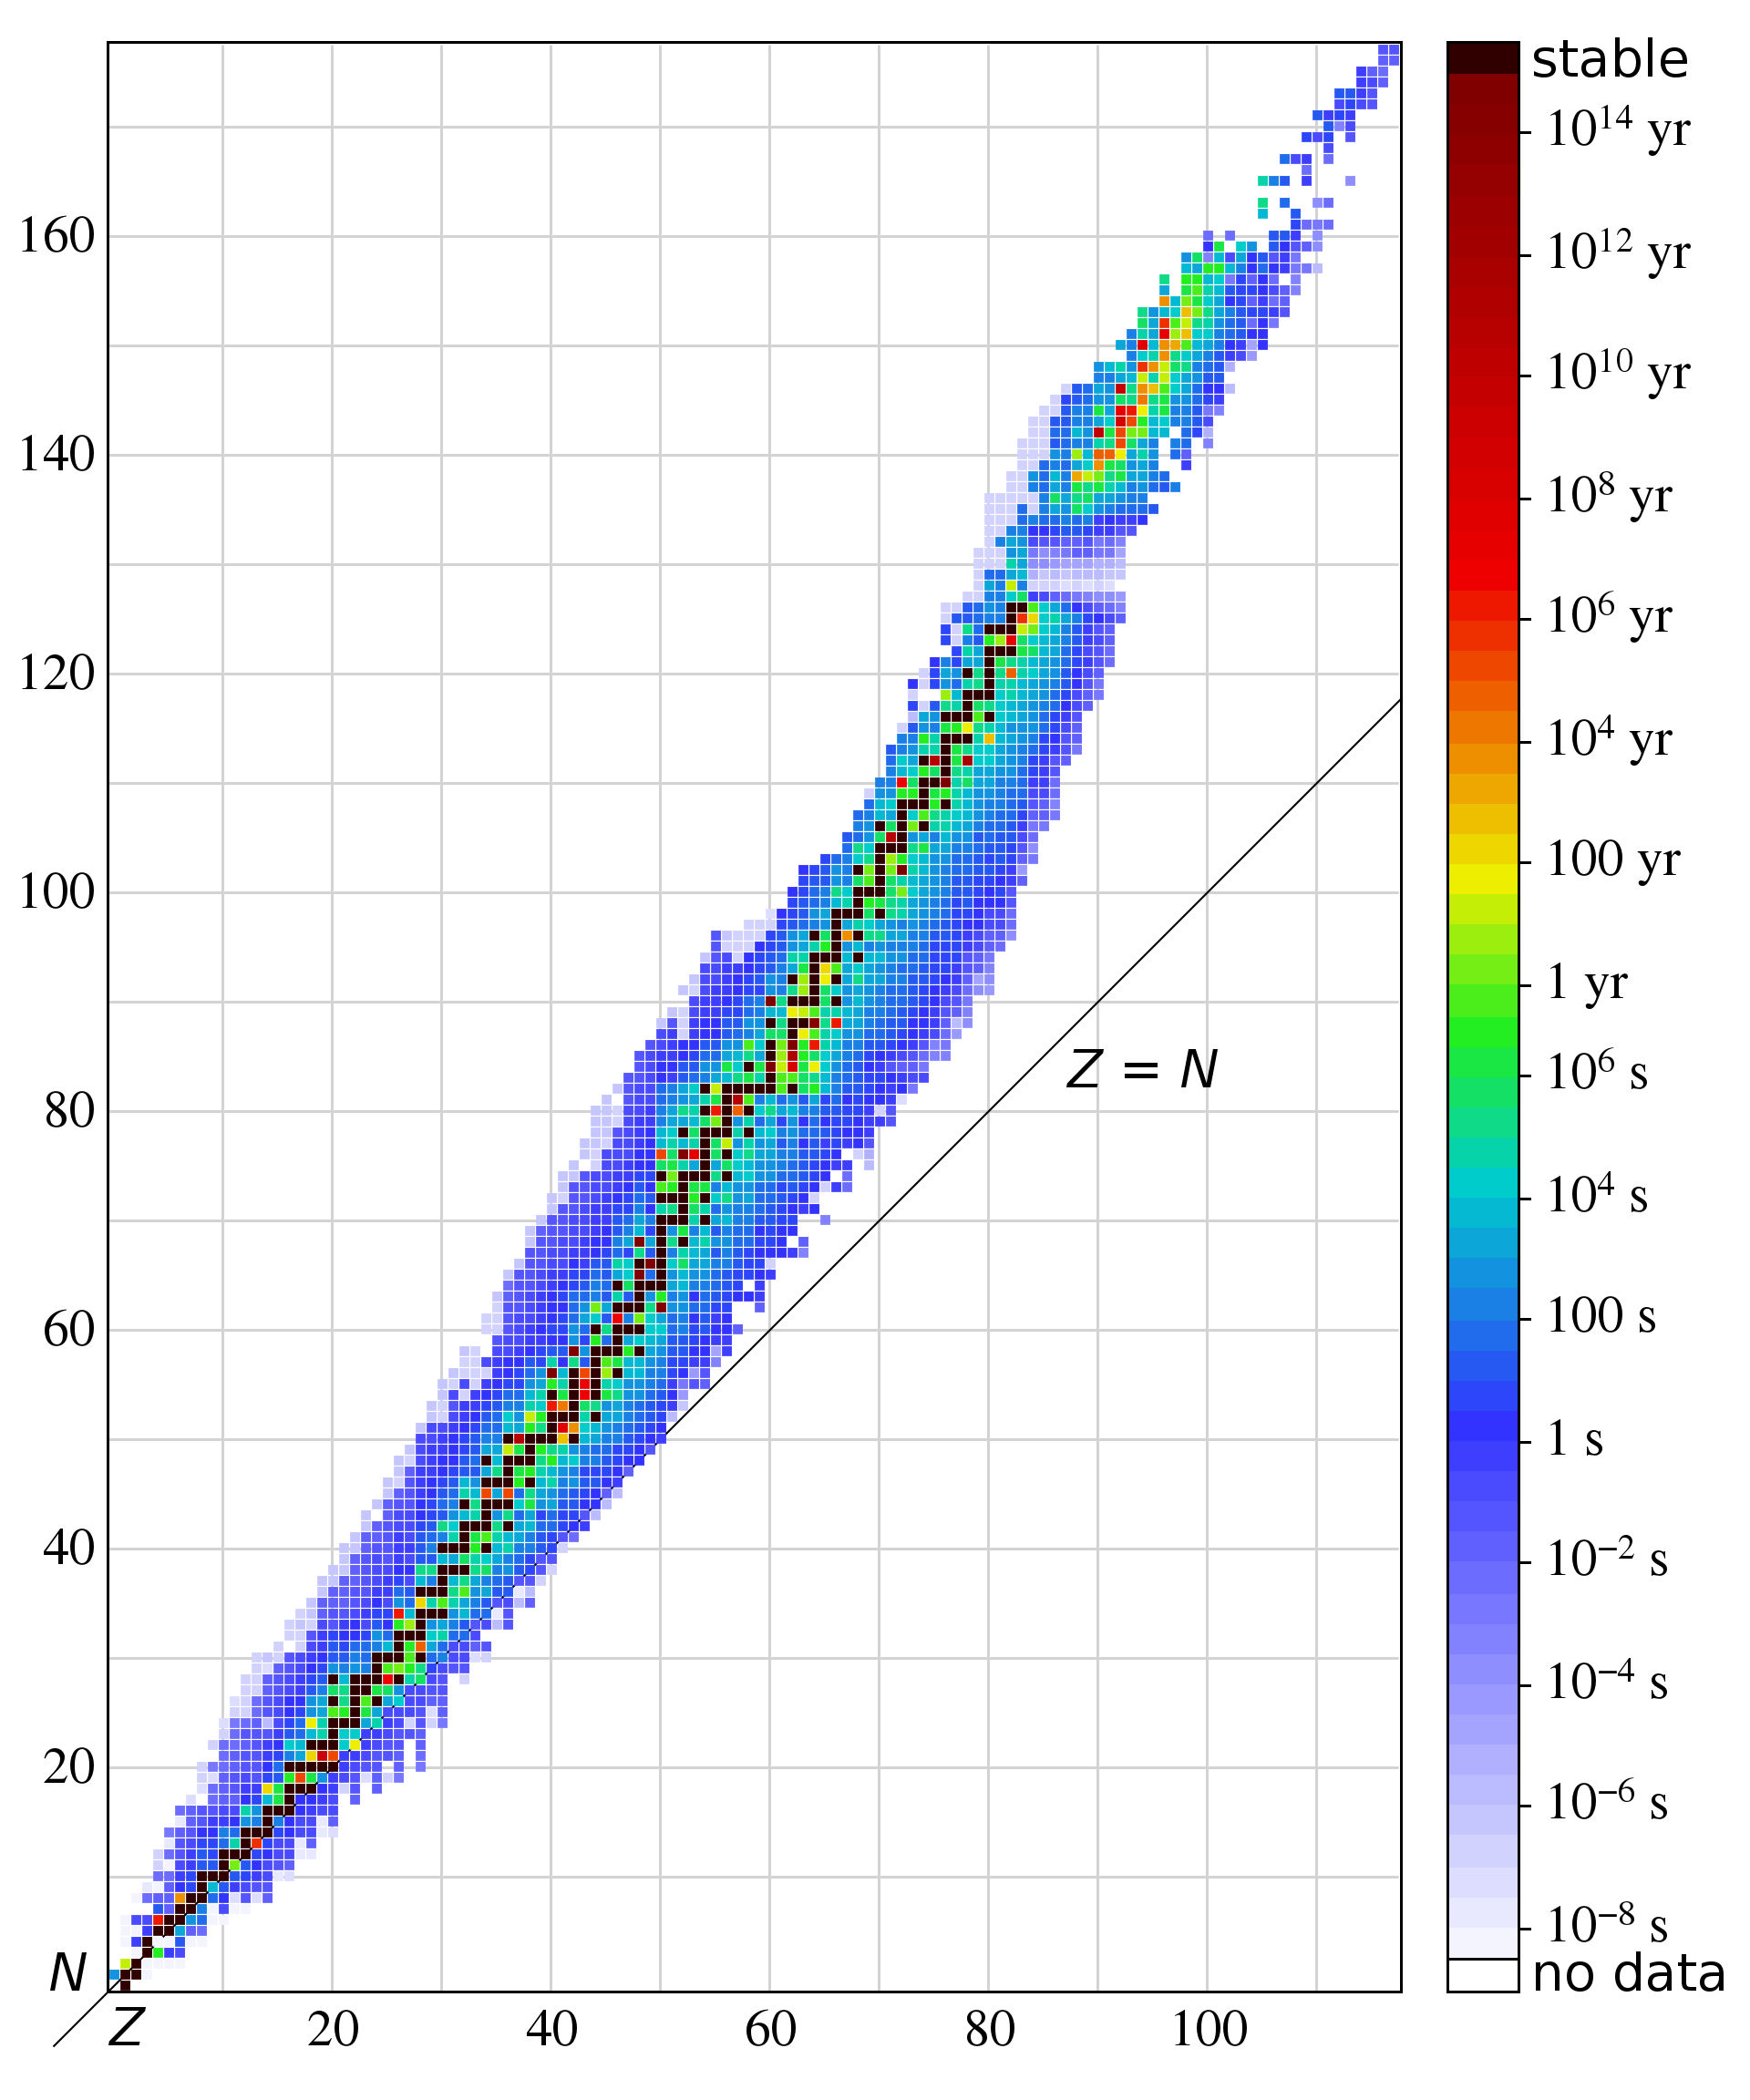
\includegraphics[width=0.8\textwidth]{images/chap1/Isotopes_and_half-life.svg.png}
    \caption{Caption .... plot from wiki}
    \label{fig:isotopes_proton_neutron_ratio}
\end{figure}

Para. 

\begin{itemize}
    \item how to define the radius (RMS)
    \item the proton distribution measurement (ep. scattering)
    \item the neutron distribution measurement is poorly 
    \item assumptions
\end{itemize}


Para.

\begin{itemize}
\item history of the nuclear structure
    \item nucleus structure, how to understand it
    \item charge radius measurement [merge with chapter 2?]
    \item scatter is used for nuclear structure probe, charge radius 
\end{itemize}


Para. 

\begin{itemize}
    \item EM force, nuclear force
    \item neutron density and assumptions
\end{itemize}


\begin{itemize}
    \item neutron charges 0, poorly measured
    \item historical measurement 
    \item parity violation measurement of the neutron density
\end{itemize} 

\section{Rich Physics Behind the PRex Experiment}
\subsection{Neutron density of neutron-rich matter}
\subsection{neutron density theory and corrections to APV}
\subsection{neutron radius measurements}
\subsection{Gravity waves, EOS, and neutron stars}
\subsection{Atomic Parity Non-Conservation Experiment}

\section{Previous Experiment}
\subsection{current theory of the neutron density}

\section{Historical measurement[to be added, move to chapter 1]}
\subsection{Pb charged radius measurement and its result }

\section{Impact of the experiment, result based on PRex-II experiment [move to chapter 6 conclusion]}

\subsection{calculate with Coulomb energy differences Phys. Lett 29B 396 (1969)}
\subsection{L. Ray and G.W.Hoffmann Physics Rev C 31. 538 (1985)}
\subsection{ Parity Violating Measurements of the Neutron Density, C.J. Horowitz, etc}
\subsection{PRex-I experiment}